\subsection{Arquitectura funcional}
La arquitectura funcional del sistema se ilustra mediante una estructura FBS
\renewcommand{\arraystretch}{0.7} % compacta filas
\begin{table}[H]
	\centering
	\caption{Funciones y subfunciones del SM}
	\begin{tabular}{l}
		\toprule
\textbf{Función principal: Preparar Cubo para Entrenamiento} \\ \hline
1.0 \; Gestionar energía \\ 
\hspace{0.5cm} 1.1 \; Obtener energía \\
\hspace{0.5cm} 1.2 \; Distribuir energía \\
\hspace{0.5cm} 1.3 \; Acondicionar energía \\ \hline
2.0 \; Gestionar información \\
\hspace{0.5cm} 2.1 \; Gestionar Interacción con Usuario\\
\hspace{1cm} 2.1.1 \; Recibir Selección de Algoritmo \\
\hspace{1cm} 2.1.2 \; Mostrar Estado del Sistema \\
\hspace{1cm} 2.1.3 \; Procesar datos \\
\hspace{0.5cm} 2.2 \; Determinar Estado del Cubo \\
\hspace{1cm} 2.2.2 \; Adquirir Datos del Cubo \\
\hspace{1cm} 2.2.3 \; Interpretar Datos \\
\hspace{1cm} 2.2.4 \; Construir Modelo Virtual \\
\hspace{0.5cm} 2.3 \; Tomar decisiones: Calcular Secuencia de Movimientos \\
\hspace{1cm} 2.3.1 \; Obtener Algoritmo Objetivo \\
\hspace{1cm} 2.3.1 \; Calcular Algoritmo Inverso \\
\hspace{1cm} 2.3.2 \; Traducir Algoritmo a Comandos \\ \hline
3.0 \; Proteger y soportar el sistema \\
\hspace{0.5cm} 3.1 \; Soporte de actuadores \\
\hspace{0.5cm} 3.2 \; Proteger cableado y dispositivos electrónicos \\\hline
4.0 \; Entorno de Visión \\
\hspace{0.5cm} 4.1 \; Posición de cámara \\
\hspace{0.5cm} 4.2 \; Posición de sensores \\
\hspace{0.5cm} 4.3 \; Iluminación \\\hline
5.0 \; Manipular Físicamente el Cubo \\
\hspace{0.5cm} 5.1 \; Sujetar Cubo \\
\hspace{0.5cm} 5.2 \; Rotar Caras \\
\hspace{0.5cm} 5.3 \; Liberar Cubo \\\hline
\end{tabular}%
\end{table}
\renewcommand{\arraystretch}{1.0} % vuelve al valor normal



\begin{figure}[H]
    \centering
    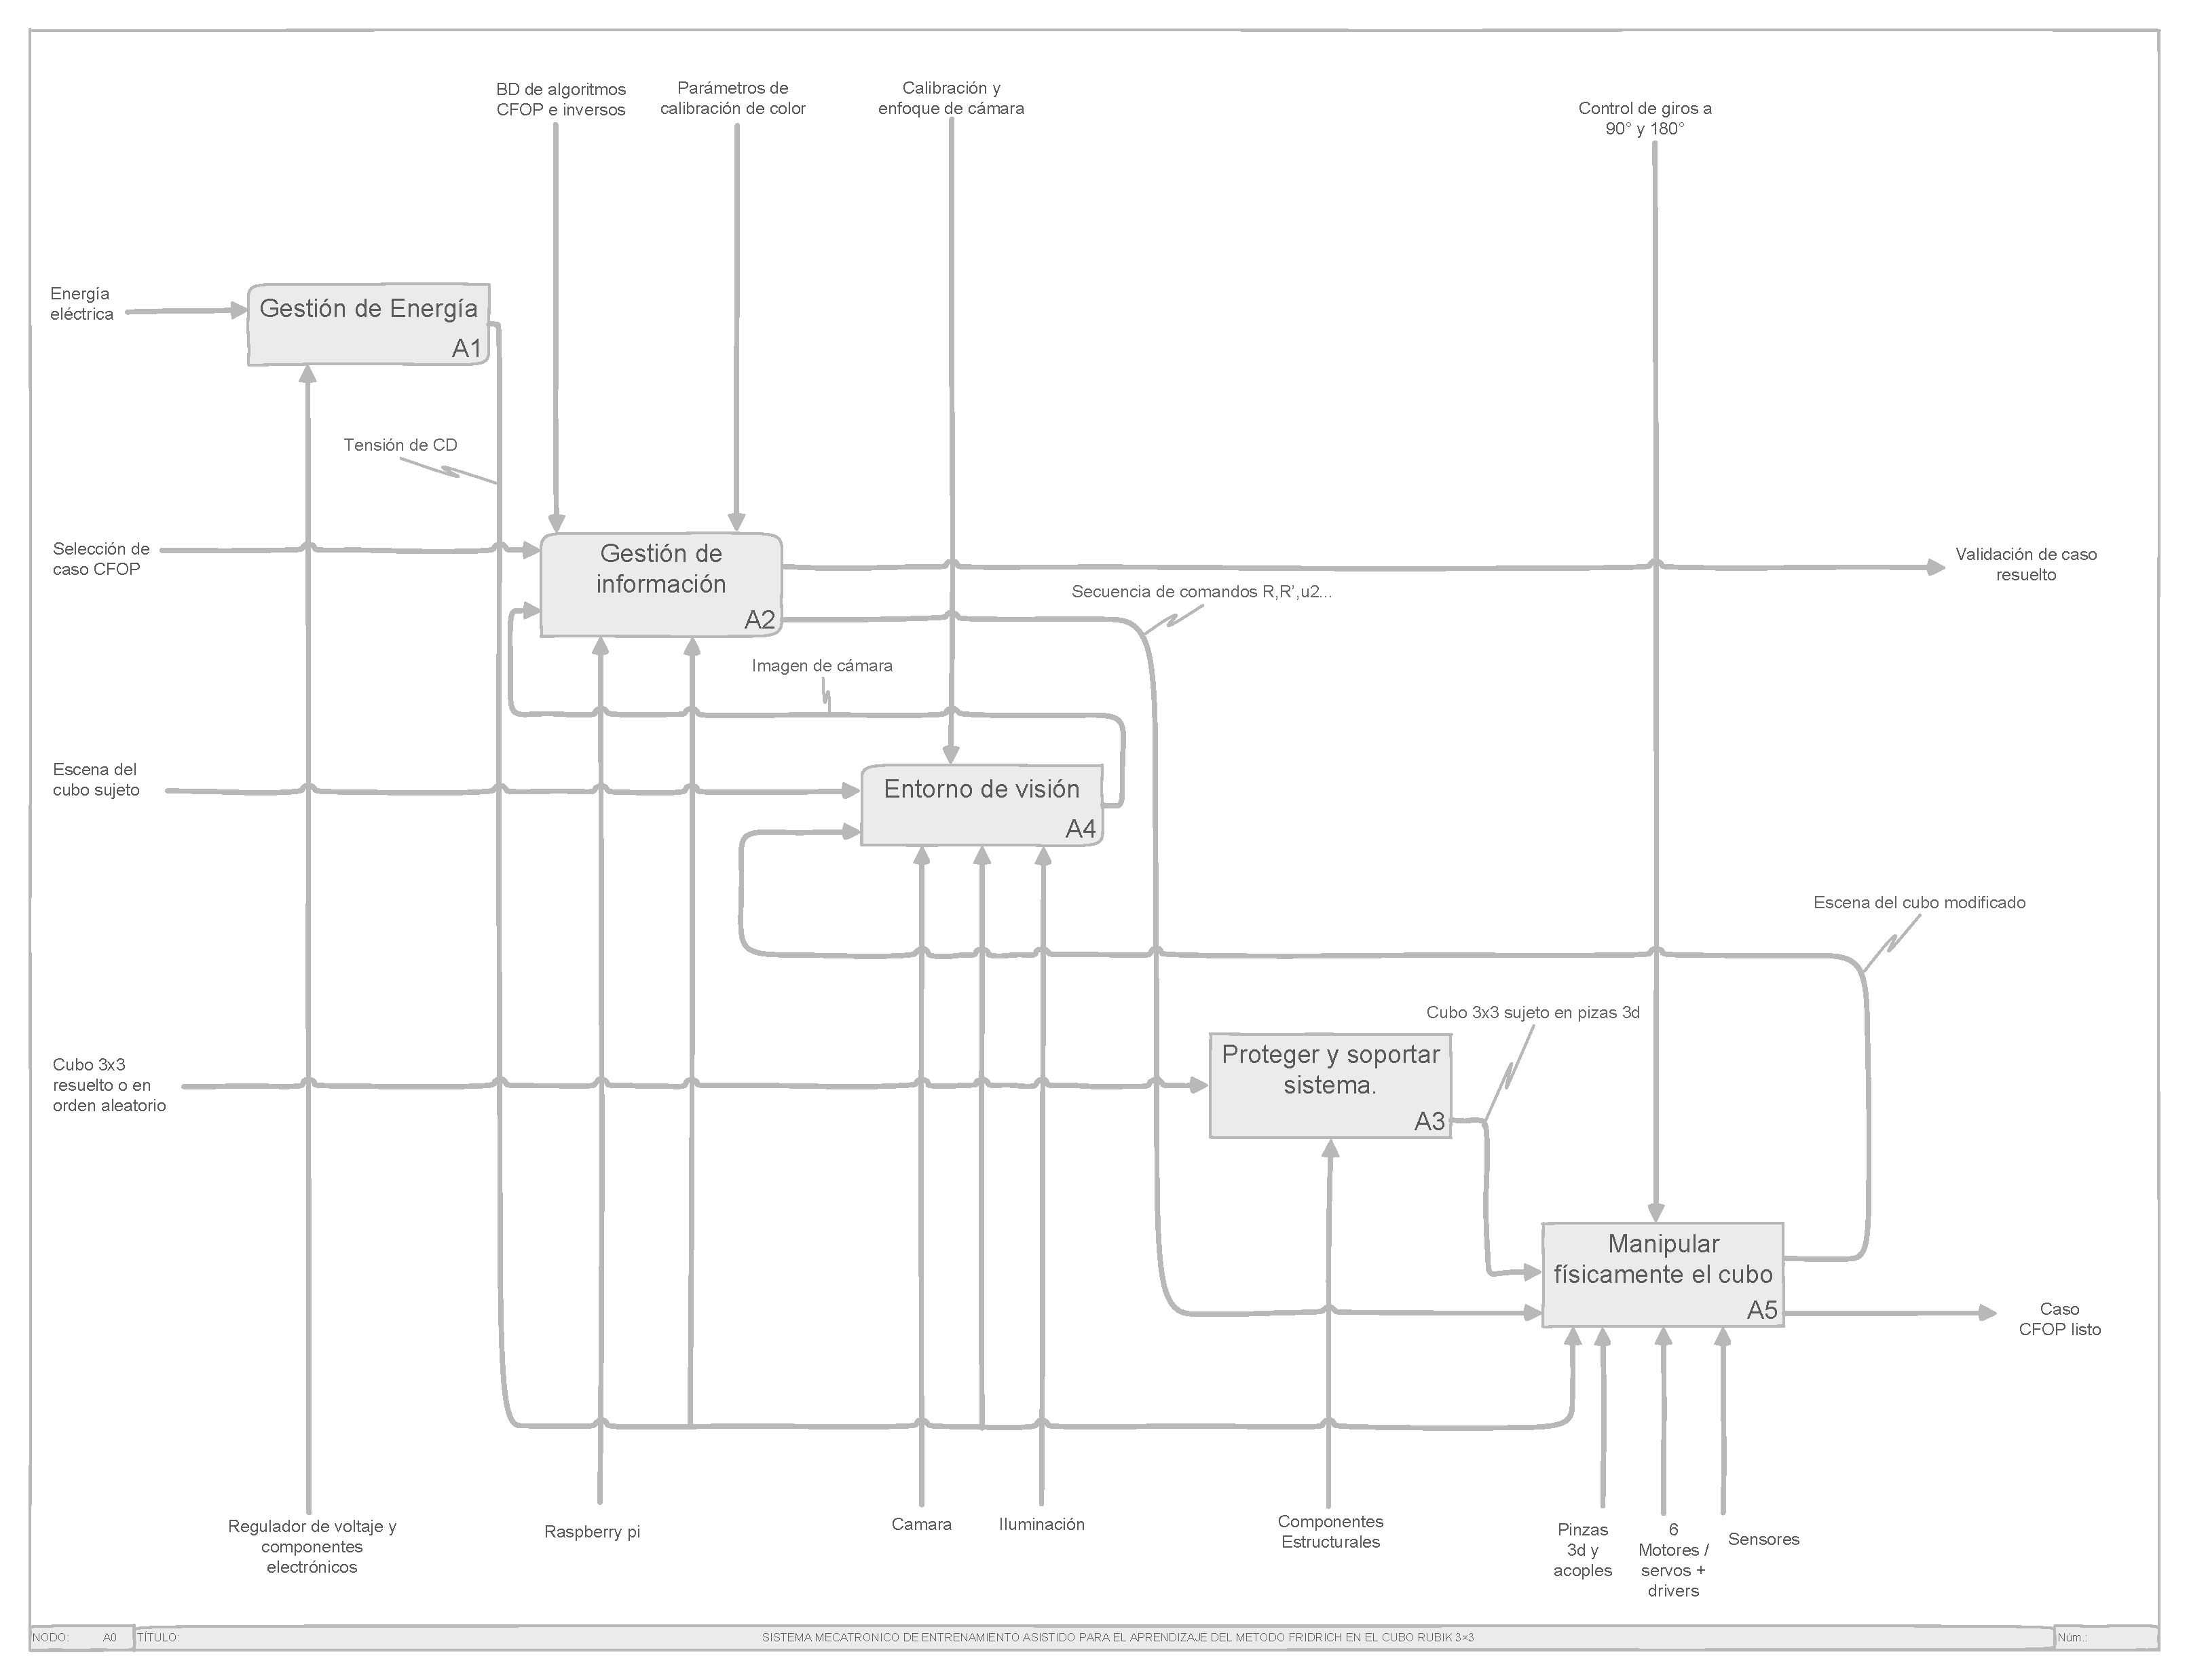
\includegraphics[height=\textwidth,angle=90]{img/idef-0-cubo.pdf} % o .png
    \caption{Diagrama IDEF-0 del cubo}
    \label{fig:idef0cubo}
\end{figure}

\\